\section{Programming Model}

\begin{figure}
\begin{center}
  \begin{ocaml}
  module type CANVAS = sig
    type pixel = {r:char; g:char; b:char}
    type tree = 
      | N of pixel
      | B of {tl: tree; tr: tree; bl: tree; br: tree} 
    type t = {max_x:int; max_y:int; canvas:tree} 
    type loc = {x:int; y:int}
  
    val new_canvas: int -> int -> t
    val set_px: t -> loc -> pixel -> t
    val get_px: t -> loc -> pixel
    val merge: (* lca *)t -> (* v1 *)t -> (* v2 *)t -> t
  end
  \end{ocaml}
\end{center}
\caption{\drawsome: a sample \name application}
\label{fig:canvas-sig}
\end{figure}

In this section, we describe the \name programming model through the
example of a collaborative drawing application we call \drawsome.

Fig.~\ref{fig:canvas-sig} shows the signature of the \drawsome
application. \drawsome represents a free-hand drawing canvas in terms
of a tree of quadrants.  Each quadrant is simply a leaf node
containing a single pixel (\C{r},\C{g}, or \C{b}) or a tree, if the
quadrant contains multiple pixels of different colors. Quadrants are
expanded into a tree structures as and when pixels are colored.  The
representation is thus optimized for sparse canvases, such as
whiteboards. The application supports three simple operations:
creating a new canvas, setting the pixel at a specified coordinate,
and returning the pixel at a given coordinate. The \C{merge} function
and \C{deriving versioned} directive are explained below.

\begin{figure}
\centering
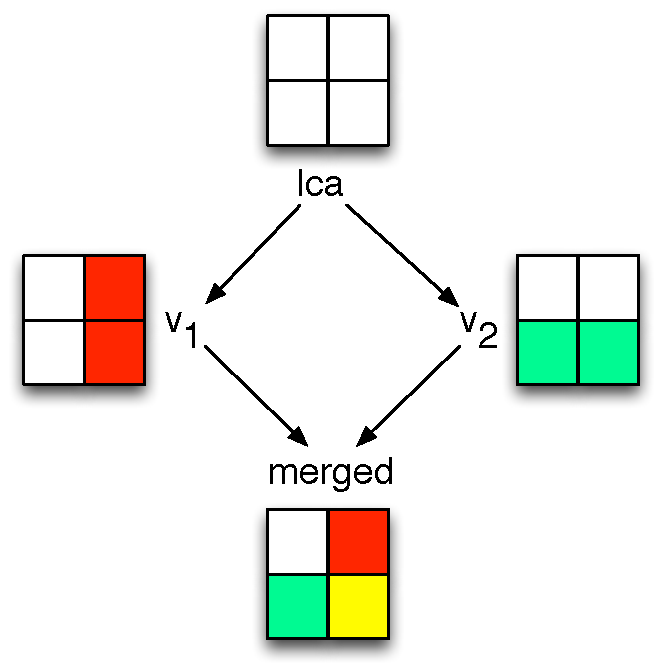
\includegraphics[scale=0.5]{Figures/canvas-merging}

\caption{Merging concurrent versions (\C{v1} and \C{v2} ) of a drawing
canvas. \C{lca} is their common ancestor.}
\label{fig:canvas-merging}
\end{figure}

\drawsome lets multiple users collaborate on a canvas that is
conceptually shared among them. Under a shared-memory abstraction,
there would be a single copy of the canvas that is updated
concurrently by multiple clients; from the perspective of any single
client, the canvas could change without any explicit
intervention. \name ascribes functional semantics to sharing by
letting each client work on its own version of the state (the tree
data structure), later merging concurrent versions on-demand.  Thus,
the primary artifact of the \name programming model is a versioned
data structure in which different versions are managed by different
clients.

%% The library operates on a representation of versioned data
%% structures optimized for persistence on disk
%% (Sec.~\ref{sec:persistence}).  \name's meta-programming component
%% automatically synthesizes this representation, along with the
%% functions that translate between representations, for the data type
%% definitions marked with the ppx~\cite{ppx} directive \C{deriving
%%   versioned}. Concretely, for the \C{Canvas} module, \name synthesizes
%% a \C{Canvas.Versioned} module with a type \C{t}, and functions
%% \C{of\_canvas} and \C{to\_canvas} of types \C{Canvas.t $\rightarrow$
%%   t} and \C{t $\rightarrow$ Canvas.t}, respectively.

\name requires a three-way \C{merge} function to merge the concurrent
versions of a drawing canvas (see Fig.~\ref{fig:merge-canvas}). The
three arguments include two concurrent versions (\C{v1} and \C{v2}),
and their least common ancestor (\C{lca}) - the version from which the
two concurrent versions evolved independently. The merge function can
make use of the pixel values of the common ancestor to merge the pixel
values on both the canvases. For instance, if the color of a pixel in
\C{v1} is white, and in \C{v2} it is green, and its color in \C{lca}
is white, then it means that only \C{v2} modified the color. Hence the
pixel is colored green in the merged canvas. On the other hand, if the
pixel is red in \C{v1}, then it means that both \C{v1} and \C{v2} have
modified the color. In such case, an appopriate color-mixing algorithm
can be used to determine the color of pixel.  For instance, the pixel
can be colored yellow - an additive combination of red and green. The
logic is illustrated in Fig.~\ref{fig:canvas-merging}.
\begin{figure}
\begin{center}
  \begin{ocaml}
let color_mix px1 px2 : pixel = 
let f = Char.code in
let h x y = Char.chr @@ (x + y)/ 2 in
let (r1,g1,b1) = (f px1.r, f px1.g, f px1.b) in
let (r2,g2,b2) = (f px2.r, f px2.g, f px2.b) in
let (r,g,b) = (h r1 r2, h g1 g2, h b1 b2) in {r=r; g=g; b=b}

let b_of_n px = B {tl_t=N px; tr_t=N px; bl_t=N px; br_t=N px}

let rec merge lca v1 v2 = 
  if v1=v2 then v1
  else if v1=lca then v2
  else if v2=lca then v1
  else match (lca,v1,v2) with
    (*
     * The first three rules isomorphize lca, v1 and v2.
     *)
    | (_, B _, N px2) -> merge lca v1 @@ b_of_n px2
    | (_, N px1, B _) -> merge lca (b_of_n px1) v2
    | (N px, B _, B _) -> merge (b_of_n px) v1 v2
    | (B x, B x1, B x2) ->
        let tl_t' = merge x.tl_t x1.tl_t x2.tl_t in
        let tr_t' = merge x.tr_t x1.tr_t x2.tr_t in
        let bl_t' = merge x.bl_t x1.bl_t x2.bl_t in
        let br_t' = merge x.br_t x1.br_t x2.br_t in
          B {tl_t=tl_t'; tr_t=tr_t'; bl_t=bl_t'; br_t=br_t'}
    | (_, N px1, N px2) -> 
        (* pixels are merged by mixing colors *)
        let px' = color_mix px1 px2 in N px'
 \end{ocaml}
\caption{Merging different versions of a canvas.}
\label{fig:merge-canvas}
\end{center}
\end{figure}

The \name programming model lets programmers define and compose
concurrent computations around versioned data structures.
Fig.~\ref{fig:dali-monad} shows the signature of the \name module that
implements the programming model along the lines of the well-known
\C{State} monad~\cite{wadler-monad}. The monad encapsulates a
versioned functional state (\C{'a}) and the type \C{('a, 'b) t}
represents a monadic computation that returns a \C{'b} result.
Functions \C{return} and \C{bind} have their usual monadic
\begin{figure}
\begin{center}
  \begin{ocaml}
  module type DALI = sig
    type ('a, 'b) t
    val return : 'b -> ('a, 'b) t
    val bind : ('a, 'b) t -> ('b -> ('a, 'c) t) -> ('a, 'c) t
    val get_current_version: unit -> ('a, 'a) t
    val with_init_version_do: 'a -> ('a, 'b) t -> 'b
    val fork_version : ('a, 'b) t -> 'a unit t
    val sync_next_version: unit -> ?v:'a -> ('a, 'a) t
  end
  \end{ocaml}
\label{fig:dali-monad}
\caption{Signature of the \name monad}
\end{center}
\end{figure}
interpretation. \C{get\_current\_version} is like the \C{State}
monad's \C{get}; it returns the versioned state encapsulated by the
monad. \C{with\_init\_version\_do} runs a monadic computation against
a given initial version and returns the result. \C{fork\_version}
returns a computation that forks a new concurrent version from the
current version, and runs the given monadic computation asynchronously
against the forked version.  \C{sync\_next\_version} (simply called
\C{sync}) accepts a \emph{proposal} for the next version of the state;
this proposal is the current local version of the state that reflects
local modifications not yet witnessed by any other concurrently
executing computation.  The operation returns (via a monad) the actual
next version, which becomes the current version for the rest of the
computation.  This version is created by merging the proposal with a
subset of concurrent versions that have become available since the
last merge or fork. Thus, \C{sync} effectively lets a computation sync
with a subset of concurrent computations to obtain their latest
updates.

\begin{figure}
\centering
\begin{tabular}{l||l||l}
\begin{ocaml}
let alice_f : C.t unit t = 
  get () >>= fun c0 -> 
  fork bob_f >>= fun () ->
  let c0' = C.draw_line c0 
    {x=0;y=0}
    {x=4;y=0} in
  sync () ~v:c0' >>= 
  fun c1 ->
  let c1' = C.draw_line c1 
    {x=0;y=4} 
    {x=4;y=4} in
  sync () ~v:c1' >>= 
  fun c2 -> return ()
\end{ocaml}
&
\begin{ocaml}
let bob_f : C.t unit t = 
  get () >>= fun c0 -> 
  fork cheryl_f >>= 
  fun () ->
  let c0' = C.draw_line c0 
    {x=0;y=0} 
    {x=0;y=4} in
  sync () ~v:c0' >>= 
  fun c1 -> sync () >>= 
  fun c2 -> return ()
\end{ocaml}
&
\begin{ocaml}
let cheryl_f : C.t unit t = 
  get () >>= fun c0 -> 
  let c0' = C.draw_line c0 
    {x=4;y=0} 
    {x=4;y=0} in
  sync () ~v:c0' >>= 
  fun c1 -> sync () >>= 
  fun c2 -> return ()
\end{ocaml}
\\
\end{tabular}
\caption{\drawsome: A collaborative drawing session between Alice,
Bob, and Cheryl}
\label{fig:canvas-sessions-code}
\end{figure}

Fig.~\ref{fig:canvas-sessions-code} demonstrates how a collaborative
drawing session between Alice, Bob and Cheryl can be composed using
\name. A possible execution of the session is visualized in
Fig.~\ref{fig:canvas-sessions}. Assume that the session starts with
Alice on a $5\times 5$ blank canvas, as shown below:
\begin{ocaml}
  module C = Canvas;; 
  with_init_version_do (C.new_blank 5 5) alice_f 
\end{ocaml}
Alice starts by reading the current version of the canvas, which is
blank. She then invites Bob for collaboration by forking a new
concurrent version for Bob. Bob, in turn, invites Cheryl for
\begin{figure}
\centering
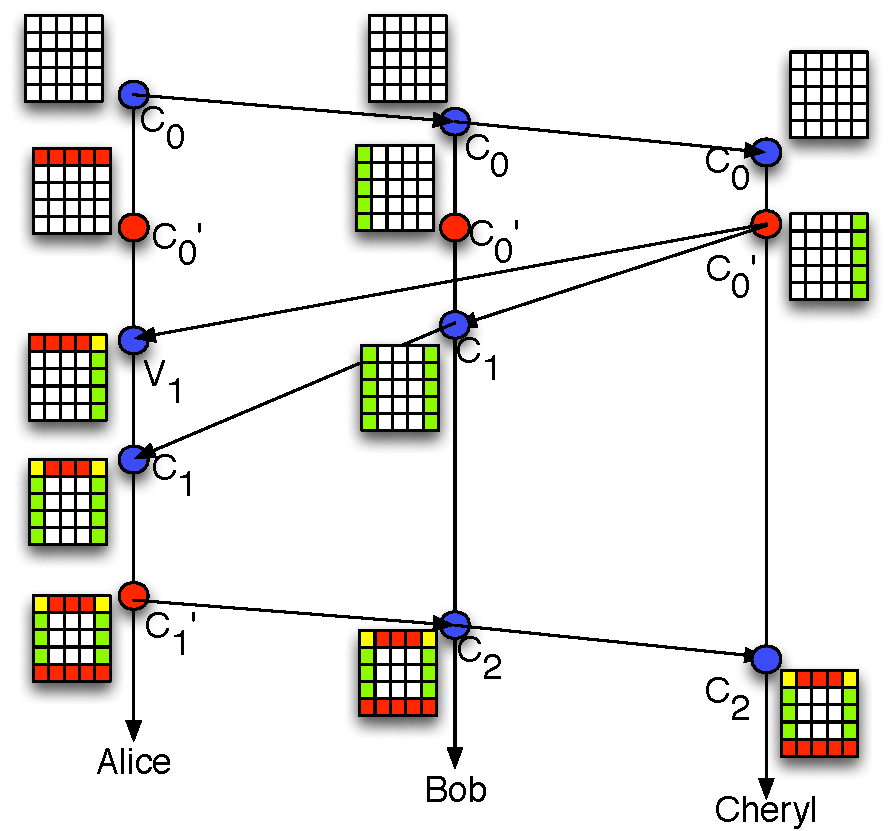
\includegraphics[scale=0.6]{Figures/canvas-sessions}
\caption{\drawsome: Collaborative drawing session visualized}
\label{fig:canvas-sessions}
\end{figure}
collaboration. All three of them start working on the blank canvas.
Alice draws a red horizontal line from $(0,0)$ (top-left) to $(4,0)$
(top-right) using \C{C.draw\_line}.\footnote{Its definitionis not
  shown, but can be constructed using \C{set\_px}} Meanwhile, Bob
draws a green vertical line from $(0,0)$ to $(0,4)$, and Cheryl draws
a similar line from $(4,0)$ to $(4,4)$. All three of them call
\C{sync} with their respective proposals ($C_0'$). While any partial
ordering of concurrent \C{syncs} is valid, we consider a linear order
where Cheryl's \C{sync} happens first, followed by Bob's and then
Alice's.  Cheryl's \C{sync} does not find any concurrent versions,
hence installs the proposed version ($C_0'$) as the next version on
Cheryl's branch. Bob's \C{sync} finds Cheryl's $C_0'$ as a concurrent
version, and merges it with its proposal to produce the next version
$C_1$, which is then installed on Bob's branch.  The least common
ancestor (LCA) for this merge is the initial version ($C_0$), and the
two concurrent versions are Bob's $C_0'$ and Cheryl's $C_0'$. Next,
Alice's \C{sync} finds Cheryl's $C_0'$ and Bob's $C_1$ as concurrent
versions, and merges them successively with Alice's proposal. For the
first merge, the two concurrent versions are Alice's $C_0'$ and
Cheryl's $C_0'$, and the LCA is the initial version ($C_0$). The
result of this merge is installed as the next version ($\C{V_1}$) on
Alice's branch. For the next merge, the two concurrent versions are
Alice's $V_1$ and Bob's $C_1$ and the LCA is Cheryl's
$C_0'$\footnote{Thus, the LCA of versions on two branches can lie
  outside both the branches.}. The result ($C_1$) becomes the next
version on Alice's branch, and the return value of Alice's \C{sync}.
Next, Alice draws a red horizontal line from $(0,4)$ to $(4,4)$,
proposes this canvas (\C{c1'} in the first column of
Fig.~\ref{fig:canvas-sessions-code}) as the next version to \C{sync}.
Since there are no concurrent versions, $C_1'$ becomes her next
version. The subsequent \C{sync} operations from Bob and Cheryl
propose no new versions, hence simply obtain Alice's $C_1'$ as next
versions.

The \drawsome example demonstrates the utility of mergeable data types
and \name programming model in building concurrent applications with
conceptual sharing of state. The model lets concurrent computations be
composed around any mergeable type. As exemplified by \drawsome,
writing a three-way \C{merge} function is the only creative process in
lifting an OCaml data type to a mergeable type. We now present few
more examples of mergeable types, and isolate a recurring pattern in
their merge functions that serves as a guide to write merge functions
for more sophisticated types.

\begin{figure}
  \centering
  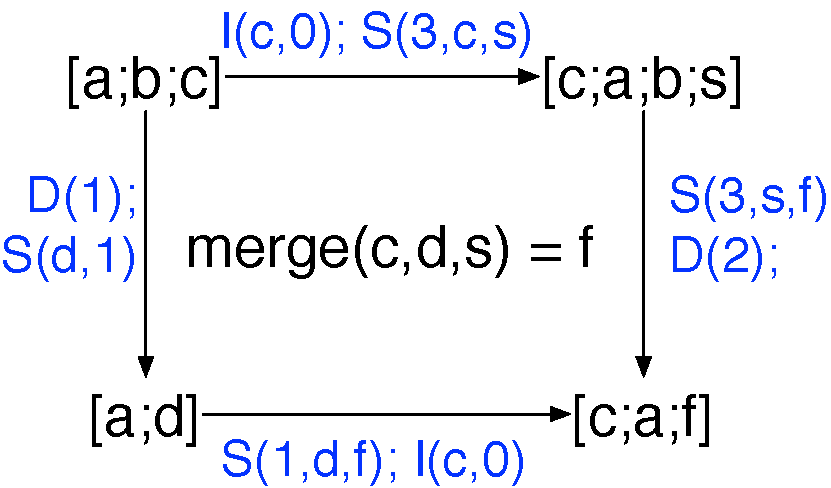
\includegraphics[scale=0.4]{Figures/list-eg}

  \caption{Lists of mergeable values are mergeable. }
  \label{fig:list-eg}
\end{figure}

\begin{figure}

\begin{subfigure}[b]{0.7\textwidth}
\begin{ocaml}
module type MList = sig
  module A: MERGEABLE
  include MERGEABLE
  type t = A.t list [@@deriving versioned]
  type edit = I of A.t * int
    | D of int
    | S of int * A.t * A.t
    | Nop
  ... (* All the standard list functions *)
  val insert: A.t -> int -> t -> t
  val delete: int -> t -> t
  val subst: int -> A.t -> t
  val edit_seq: t -> t -> edit list option
  val op_transform: edit list -> edit list -> edit list
  val merge: t -> t -> t -> t
end
\end{ocaml}
\caption{Signature of Mergeable Lists}
\label{fig:mlist-sig}
\end{subfigure}

\begin{subfigure}{0.75\textwidth}
\begin{ocaml}
(*
 * We reduce the problem of transforming op1* w.r.t op2* 
 * first to the problem of transforming op1* w.r.t op2,
 * and then to the problem of transforming op1 w.r.t op2.
*)
let op_transform mine others = 
  (*
   * Transforms my edit w.r.t other edit, and also returns how 
   * edits following my edit will witness the other edit.
   *)
  let xform my other = 
    let f my' = (my',other) in
    let g other' = (my,other') in
      match (my,other)  with 
      | (I (x,j), I (_,i)) when (j>=i) -> f @@ I (x,j+1)
      | (D j, I (_,i)) when (j>=i) -> f @@ D (j+1)
      | (S (j,x,y), I (_,i)) when (j>=i) -> f @@ S (j+1,x,y)
      | (I (x,j), D i) when (j=i) ->  g @@ Nop
      | (I (x,j), D i) when (j>i) ->  f @@ I (x,j-1)
      | (D j, D i) when (j=i) -> (Nop, Nop)
      | (D j, D i) when (j>i) ->  f @@ D (j-1)
      | (S (j,x,y), D i) when (j=i) -> f @@ Nop
      | (S (j,x,y), D i) when (j>i) -> f @@ S (j-1,x,y)
      | (I (x,j), S (i,y,z)) when (j<=i) -> g @@ S (i+1,y,z)
      | (D j, S (i,y,z)) when (j=i) -> g @@ Nop
      | (D j, S (i,y,z)) when (j<i) -> g @@ S (i-1,y,z)
      | (S (j,x,y), S (i,_,z)) when (j=i) -> f @@ S (j,x,A.merge x y z) 
      | _ -> f @@ my in
  let mine' = 
    List.fold_left 
      (fun mine other -> 
         let (mine',_) = 
           List.fold_left 
             (fun (xformed, other) my -> 
                let (my',other') = xform my other in
                  (xformed@[my'],other')) 
             ([],other) mine in
           mine') 
      mine others in
    mine'
\end{ocaml}
\caption{Operational transformation of list operations}
\label{fig:mlist-xform}
\end{subfigure}

\caption{Mergeable List Implementation}
\label{fig:mlist}
\end{figure}


{\bf Lists}. List, as an abstract data type, supports three
operations: \C{insert x i l}, that inserts an element \C{x} at
position \C{i} in the list \C{l}, \C{delete i l}, that deletes the
element at \C{i}'th position, and \C{subst i x l}, that substitutes
the element at \C{i}'th position with \C{x}. Lists of mergeable items
are mergeable. The signature of a mergeable list library is shown in
Fig.~\ref{fig:mlist-sig}. Note that the type of items in the list
(\C{A.t}) is also required to be mergeable. The signature
\C{MERGEABLE} will be discussed shortly. 

The merge operation for lists is composed of two separate functions,
\C{edit\_seq} and \C{op\_transform}.
\begin{itemize}
  \item \C{edit\_seq} takes a pair of lists, \C{v} and $\C{v'}$, and
  computes the shortest sequence of list operations that need to be
  applied on \C{v} to obtain \C{v'}. Such a sequence is called an
  \emph{edit sequence}. The length of the sequence corresponds to the
  standard notion of the \emph{edit distance} between the two lists,
  which can be computed in polynomial time, for e.g., using the
  Wagner-Fisher algorithm~\cite{wagner-fischer}. A slight modification
  of Wagner-Fischer also lets us compute the edit sequence. The
  implementation in Fig.~\ref{fig:mlist} represents edits using the
  type \C{edit}. Constructors \C{I}, \C{D}, and \C{S} stand for
  \C{insert}, \C{delete}, and \C{subst}, respectively; \C{Nop} is
  there for technical reasons. The subst constructor also carries the
  \C{A.t} element that was substituted. Our implementation of
  Wagner-Fischer is more-or-less standard (hence, not shown), except
  that the edit sequence it returns orders \C{I}'s and \C{D}'s before
  \C{S}'s.  Fig.~\ref{fig:list-eg} illustrates edit sequences for a
  sample list. The sequence \C{[I(c,0); S(3,c,s)]} maps the list
  \C{[a;b;c]} to \C{[c;a;b;s]} because \C{subst 3 s (insert c 0
  [a;b;c]) = [c;a;b;s]}.
  \item  \C{op\_transform} takes a pair of edit sequences, $s_1$ and
  $s_2$, that map a list $v$ to two different lists, $v_1$ and $v_2$
  (e.g., Fig.~\ref{fig:list-eg}), and transforms $s_1$ to $s_1'$ such
  that $s_1'$ has the same effect on $v_2$ as $s_1$ had on $v$.  For
  instance, in Fig.~\ref{list-eg}, let $s_1$ be the edit sequence
  \C{[D(1); S(d,1)]}, which maps the list \C{[a;b;c]} ($v$) to
  \C{[a;d]} ($v_1$). The \C{D} edit deletes the first element of $v$.
  However, if $s_1$ is to be applied on the list \C{[c;a;b;s]}
  ($v_2$), which has a new element at position 0, the \C{D} edit must
  delete the the second element from $v_2$, if it were to have the
  same effect as it did on $v$. We say \C{D(1)} in $s_1$ has to be
  transformed w.r.t the sequence $s_2 = \C{[I(c,0);S(3,c,s)]}$.  The
  function \C{op\_transform} of Fig.~\ref{fig:mlist-xform} computes
  such \emph{operational transformation} for the sequence \C{mine}
  w.r.t the sequence \C{others}, and returns \C{mine'}, the
  transformed sequence. To do so, it first pulls the \C{S} edits in
  \C{mine} to the beginning of the sequence, transforming them w.r.t
  the \C{I} and \C{D} edits in \C{mine}. Having all the \C{S} edits at
  the beginning of the \C{mine} sequence makes their transformation
  easier since the offset of the transformed substitution depends only
  on the edits in the \C{other} sequence. Furthermore, it facilitates
  an easy comparison with \C{S} edits at the end of \C{other}. Next,
  \C{op\_transform} transforms edits in \C{mine} w.r.t \C{other} by
  comparing their offsets; the rules are straightforward.
\end{itemize}


This example, however, implicitly makes certain assumptions
about the model and the underlying system, such as the existence of a
single least common ancestor (LCA) for any pair of versions, the
ability to access a previous version on any branch, and mergeability
of any two concurrent versions. Enforcing these guarantees in a fully
decentralized distributed setting requires addressing non-trivial
theoretical challenges described in the next section. Unlike the
canvas, the process of writing merge functions for data types with
non-trivial invariants could be quite involved. The following sections
describe a principled approach to deriving merge functions for any
data type given its invariants. Like \C{Canvas.merge}, merge functions
often need to compare multiple versions of a data type for structural
equality, which, when performed naively, incurs cost linear in the
size of versions. The representation of a versioned data type in \name
is optimized for performing comparisons that allows structural
equality to be determined in constant time. Such engineering details,
which contribute to the practicality of our programming model are also
discussed in subsequent sections.

